\chapter{Aufgabe 2}
\textit{Nutzen Sie die integrierte Zeitmessroutine um ihren Fortschritt bei der Optimierung zu bewerten.}\\

Wir haben den Aufruf der Zeitmessung geringfügig angepasst, siehe Abbildung \ref{figureZeitmessung}. Ziel ist es die Auswertung zu vereinfachen. Um die Matrixmultiplikation zu starten, haben wir ein Skript geschrieben. Dieses Skript ist in Abbildung \ref{FigureSkript} angegeben. Dieses Skript wurde mittels $sbatch$ gestartet. 

In Abbildung \ref{gcc0} sieht man die benötigten Zeiten, für die Kompilierung mit gcc und in Abbildung \ref{icc0} die Zeiten für den Intel Compiler. Berechnungen welche länger als 30 Sekunden benötigen werden ignoriert. Alle Zeiten können im Anhang nachgeschlagen werden. Die GFLOP/s können in Abbildung \ref{Ggcc0} und in Abbildung \ref{Gicc0} abgebildet.

Zuerst betrachten wir die Zeiten des gcc compilierten Quelltextes. Durch das herausziehen der Indexberechnung und die transponierung der Matrix $B$, sinkt die benötigte Zeit auf rund ein drittel. Die GFLOP/s steigen von 0,25 auf 0,82. Der Abfall der Performance erfolgt später und weniger ausgeprägt. Bei einer Matrixgröße von 2048 unterscheiden sich die GFLOP/s um den Faktor 20. Das Ausrollen der inneren Schleife bringt zusätzlich einen Geschwindigkeitsgewinn. Die GFLOP/s steigen auf bis zu 1,5. Das Tiling ist langsamer als die Ausrollung. Die Optimierung Tiling hat maximal 1,44 GFLOP/s. Ein mögliche Erklärung ist, dass die gewählte Blockgröße schlecht ist.

Der Intel Compiler liefert Ergebnisse die vergleichbar, mit denen des gcc, sind. 

\lstset{language=c}
\begin{figure}[h]
\begin{lstlisting}
// Nothing
t_start = gtod();
mat_mult_non_opt(A,B,C, dim);
t_end = gtod();
gflops = ( ( double )2 * dim * dim * dim / 1000000000.0 ) / ( t_end - t_start );
printf("%d;%0.4f;%0.2f;", dim, t_end - t_start, gflops );
free( C );

// Transpose
C = zero_mat( dim );
t_start = gtod();
mat_mult_transpose(A,B,C, dim);
t_end = gtod();
gflops = ( ( double )2 * dim * dim * dim / 1000000000.0 ) / ( t_end - t_start );
printf("%0.4f;%0.2f;",  t_end - t_start, gflops );
free( C );

// Unroll 32 Transpose
C = zero_mat( dim );
t_start = gtod();
mat_mult_unroll_transpose(A,B,C, dim);
t_end = gtod();
gflops = ( ( double )2 * dim * dim * dim / 1000000000.0 ) / ( t_end - t_start );
printf("%0.4f;%0.2f;", t_end - t_start, gflops );
free( C );

// Unroll 32 BLOCKING
C = zero_mat( dim );
t_start = gtod();
mat_mult_blocking(A,B,C, dim);
t_end = gtod();
gflops = ( ( double )2 * dim * dim * dim / 1000000000.0 ) / ( t_end - t_start );
printf("%0.4f;%0.2f;\n", t_end - t_start, gflops );
\end{lstlisting}
\caption{Quelltext der die Veränderung der Zeitmessroutine darstellt}
\label{figureZeitmessung}
\end{figure}



\begin{figure}
\begin{lstlisting}[language=bash]
#!/bin/bash
#SBATCH --time=01:00:00
#SBATCH --partition=sandy
#SBATCH --cpus-per-task=1
#SBATCH --gres=gpu:0

module load gcc
module load intel

gcc -O0 -std=c99 ./main.c
./a.out > gccO0.csv
icc -O0 -std=c99 ./main.c
./a.out > iccO0.csv
\end{lstlisting}
\caption{Dieses Skript wird benutzt um den Auftrag auf Taurus zu starten.}
\label{FigureSkript}
\end{figure}



\begin{figure}[h]
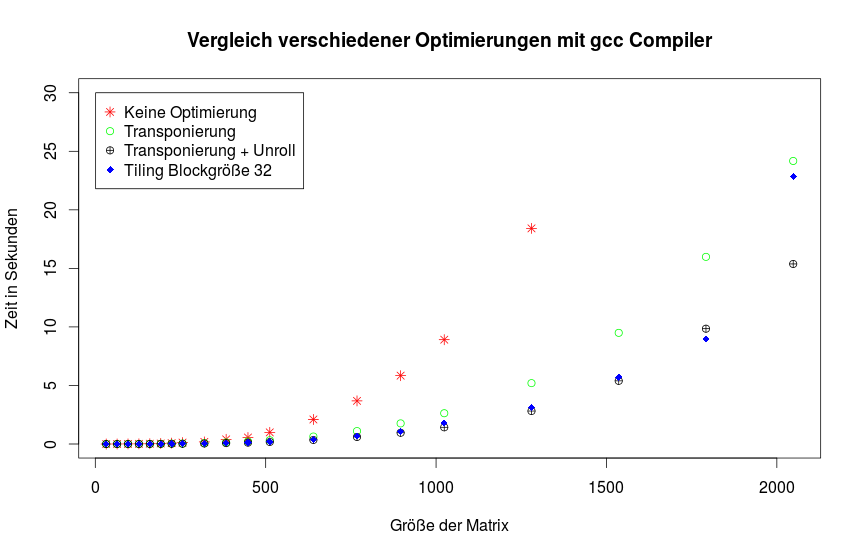
\includegraphics[scale = 0.45]{Bilder/gccO0.png}
\caption{Vergleich der Laufzeiten verschiedener Optimierungen mit dem gcc Compiler. Der Quelltext wurde mit den Parametern -O0 -std=c99 compiliert.}
\noindent\rule{14cm}{0.4pt}
\label{gcc0}
\end{figure}

\begin{figure}[h]
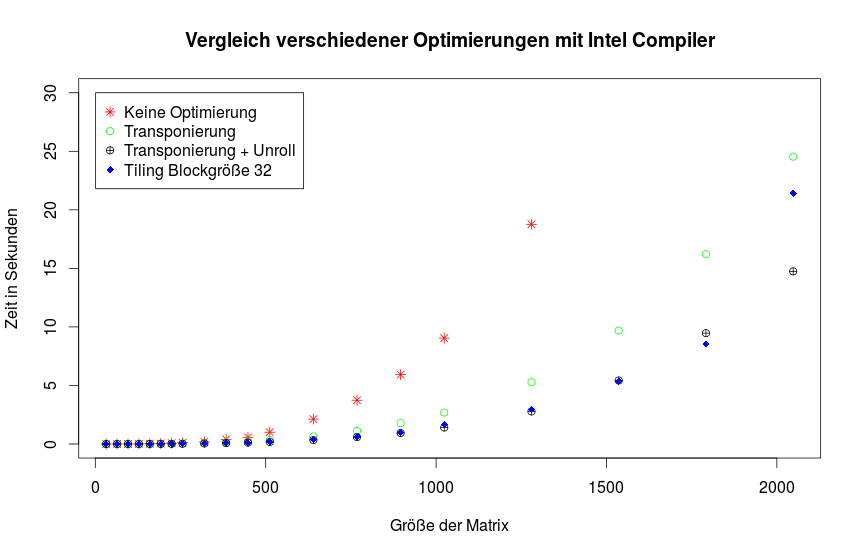
\includegraphics[scale = 0.45]{Bilder/iccO0.png}
\caption{Vergleich der Laufzeiten verschiedener Optimierungen mit dem Intel Compiler. Der Quelltext wurde mit den Parametern -O0 -std=c99 compiliert.}
\noindent\rule{14cm}{0.4pt}
\label{icc0}
\end{figure}

\begin{figure}[h]
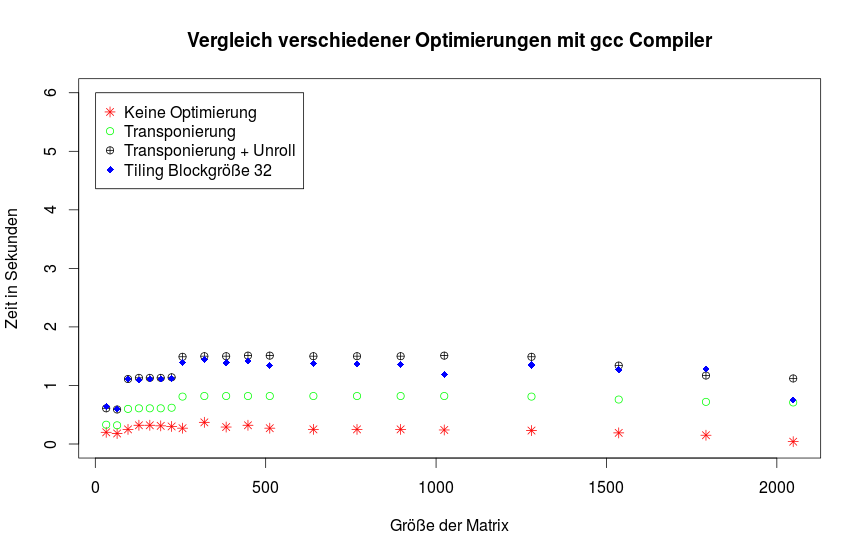
\includegraphics[scale = 0.45]{Bilder/GggcO0.png}
\caption{Vergleich der GFLOP/s verschiedener Optimierungen mit dem gcc Compiler. Der Quelltext wurde mit den Parametern -O0 -std=c99 compiliert.}
\noindent\rule{14cm}{0.4pt}
\label{Ggcc0}
\end{figure}

\begin{figure}[h]
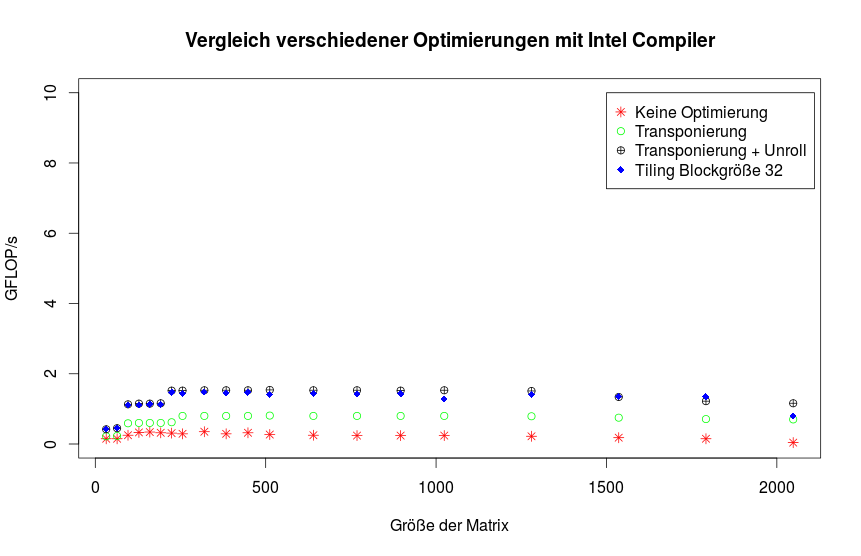
\includegraphics[scale = 0.45]{Bilder/GiccO0.png}
\caption{Vergleich der GFLOP/s verschiedener Optimierungen mit dem Intel Compiler. Der Quelltext wurde mit den Parametern -O0 -std=c99 compiliert.}
\noindent\rule{14cm}{0.4pt}
\label{Gicc0}
\end{figure}